\documentclass[1p]{elsarticle_modified}
%\bibliographystyle{elsarticle-num}

%\usepackage[colorlinks]{hyperref}
%\usepackage{abbrmath_seonhwa} %\Abb, \Ascr, \Acal ,\Abf, \Afrak
\usepackage{amsfonts}
\usepackage{amssymb}
\usepackage{amsmath}
\usepackage{amsthm}
\usepackage{scalefnt}
\usepackage{amsbsy}
\usepackage{kotex}
\usepackage{caption}
\usepackage{subfig}
\usepackage{color}
\usepackage{graphicx}
\usepackage{xcolor} %% white, black, red, green, blue, cyan, magenta, yellow
\usepackage{float}
\usepackage{setspace}
\usepackage{hyperref}

\usepackage{tikz}
\usetikzlibrary{arrows}

\usepackage{multirow}
\usepackage{array} % fixed length table
\usepackage{hhline}

%%%%%%%%%%%%%%%%%%%%%
\makeatletter
\renewcommand*\env@matrix[1][\arraystretch]{%
	\edef\arraystretch{#1}%
	\hskip -\arraycolsep
	\let\@ifnextchar\new@ifnextchar
	\array{*\c@MaxMatrixCols c}}
\makeatother %https://tex.stackexchange.com/questions/14071/how-can-i-increase-the-line-spacing-in-a-matrix
%%%%%%%%%%%%%%%

\usepackage[normalem]{ulem}

\newcommand{\msout}[1]{\ifmmode\text{\sout{\ensuremath{#1}}}\else\sout{#1}\fi}
%SOURCE: \msout is \stkout macro in https://tex.stackexchange.com/questions/20609/strikeout-in-math-mode

\newcommand{\cancel}[1]{
	\ifmmode
	{\color{red}\msout{#1}}
	\else
	{\color{red}\sout{#1}}
	\fi
}

\newcommand{\add}[1]{
	{\color{blue}\uwave{#1}}
}

\newcommand{\replace}[2]{
	\ifmmode
	{\color{red}\msout{#1}}{\color{blue}\uwave{#2}}
	\else
	{\color{red}\sout{#1}}{\color{blue}\uwave{#2}}
	\fi
}

\newcommand{\Sol}{\mathcal{S}} %segment
\newcommand{\D}{D} %diagram
\newcommand{\A}{\mathcal{A}} %arc


%%%%%%%%%%%%%%%%%%%%%%%%%%%%%5 test

\def\sl{\operatorname{\textup{SL}}(2,\Cbb)}
\def\psl{\operatorname{\textup{PSL}}(2,\Cbb)}
\def\quan{\mkern 1mu \triangleright \mkern 1mu}

\theoremstyle{definition}
\newtheorem{thm}{Theorem}[section]
\newtheorem{prop}[thm]{Proposition}
\newtheorem{lem}[thm]{Lemma}
\newtheorem{ques}[thm]{Question}
\newtheorem{cor}[thm]{Corollary}
\newtheorem{defn}[thm]{Definition}
\newtheorem{exam}[thm]{Example}
\newtheorem{rmk}[thm]{Remark}
\newtheorem{alg}[thm]{Algorithm}

\newcommand{\I}{\sqrt{-1}}
\begin{document}

%\begin{frontmatter}
%
%\title{Boundary parabolic representations of knots up to 8 crossings}
%
%%% Group authors per affiliation:
%\author{Yunhi Cho} 
%\address{Department of Mathematics, University of Seoul, Seoul, Korea}
%\ead{yhcho@uos.ac.kr}
%
%
%\author{Seonhwa Kim} %\fnref{s_kim}}
%\address{Center for Geometry and Physics, Institute for Basic Science, Pohang, 37673, Korea}
%\ead{ryeona17@ibs.re.kr}
%
%\author{Hyuk Kim}
%\address{Department of Mathematical Sciences, Seoul National University, Seoul 08826, Korea}
%\ead{hyukkim@snu.ac.kr}
%
%\author{Seokbeom Yoon}
%\address{Department of Mathematical Sciences, Seoul National University, Seoul, 08826,  Korea}
%\ead{sbyoon15@snu.ac.kr}
%
%\begin{abstract}
%We find all boundary parabolic representation of knots up to 8 crossings.
%
%\end{abstract}
%\begin{keyword}
%    \MSC[2010] 57M25 
%\end{keyword}
%
%\end{frontmatter}

%\linenumbers
%\tableofcontents
%
\newcommand\colored[1]{\textcolor{white}{\rule[-0.35ex]{0.8em}{1.4ex}}\kern-0.8em\color{red} #1}%
%\newcommand\colored[1]{\textcolor{white}{ #1}\kern-2.17ex	\textcolor{white}{ #1}\kern-1.81ex	\textcolor{white}{ #1}\kern-2.15ex\color{red}#1	}

{\Large $\underline{12n_{0488}~(K12n_{0488})}$}

\setlength{\tabcolsep}{10pt}
\renewcommand{\arraystretch}{1.6}
\vspace{1cm}\begin{tabular}{m{100pt}>{\centering\arraybackslash}m{274pt}}
\multirow{5}{120pt}{
	\centering
	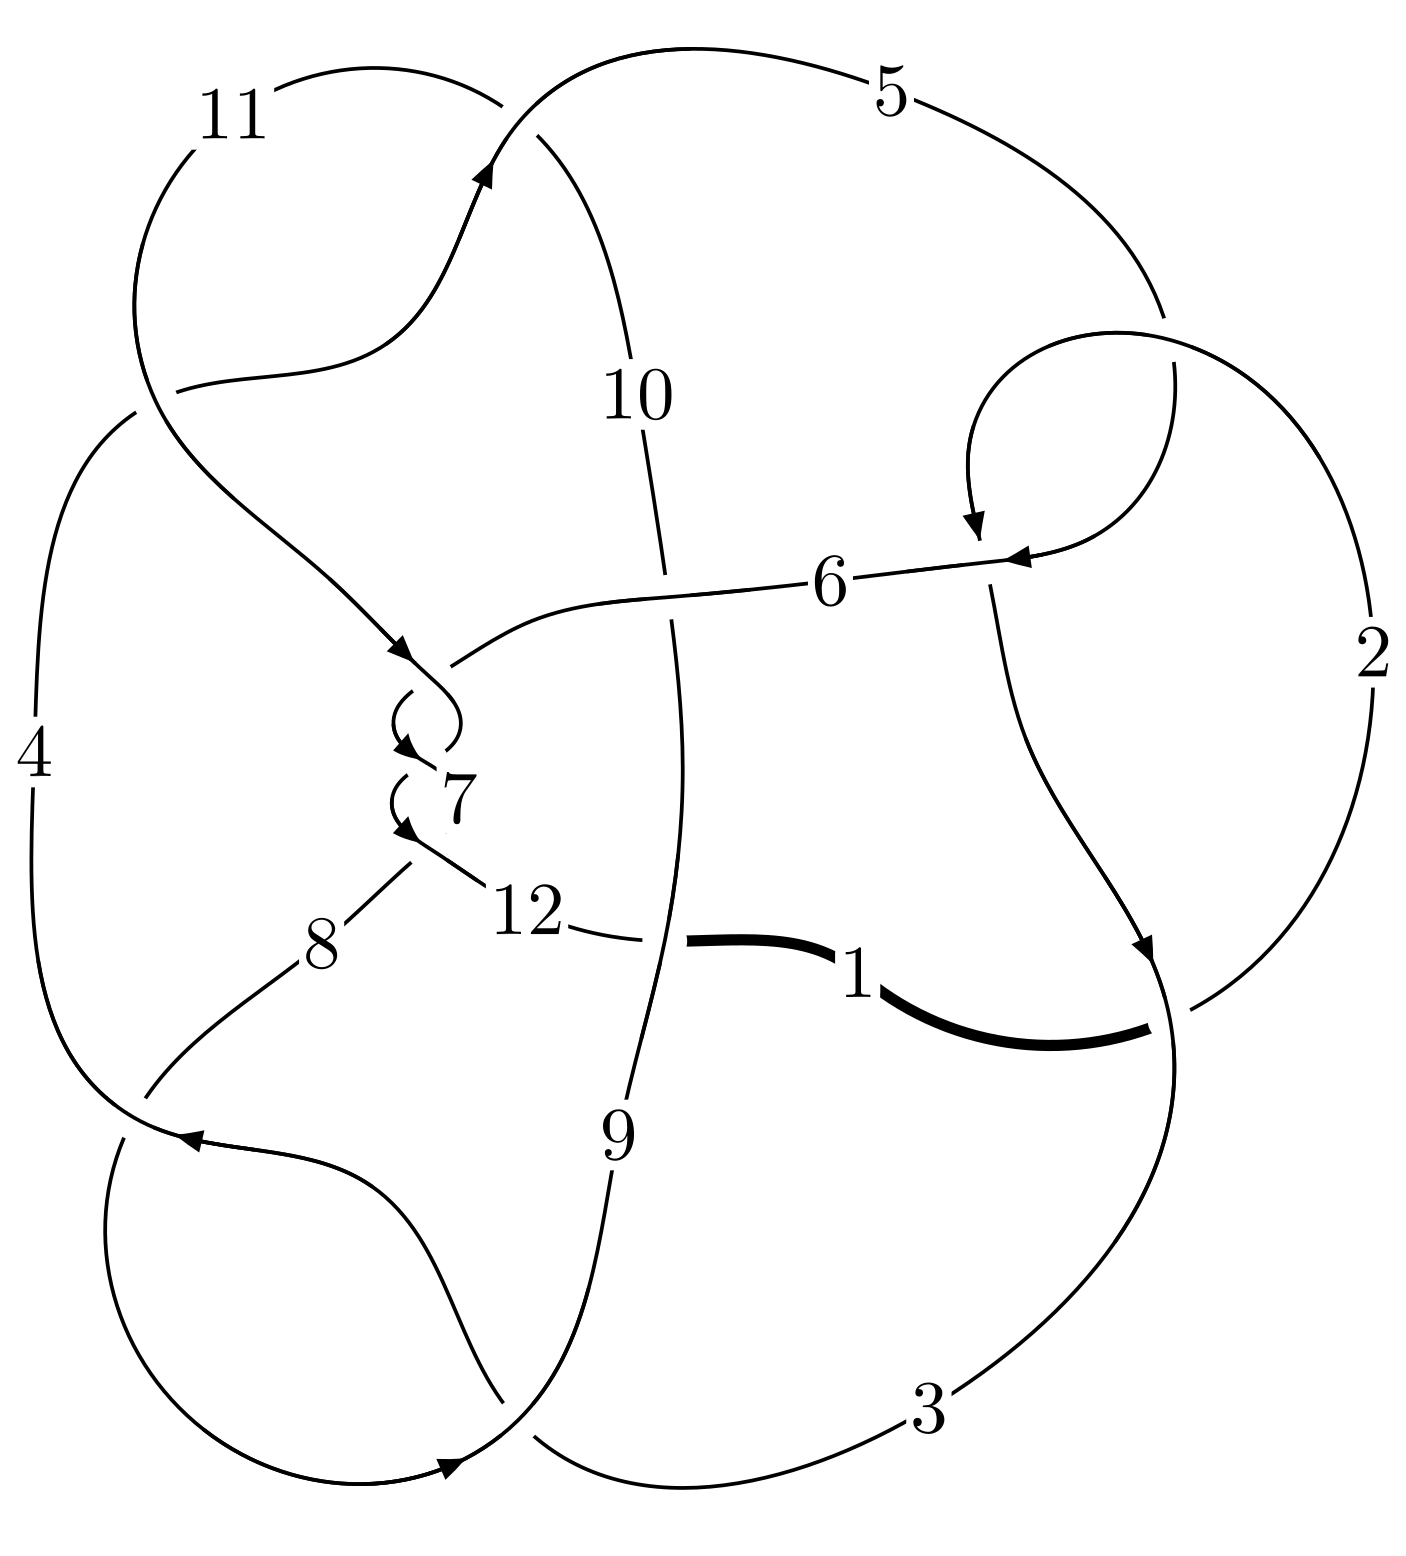
\includegraphics[width=112pt]{../../../GIT/diagram.site/Diagrams/png/2577_12n_0488.png}\\
\ \ \ A knot diagram\footnotemark}&
\allowdisplaybreaks
\textbf{Linearized knot diagam} \\
\cline{2-2}
 &
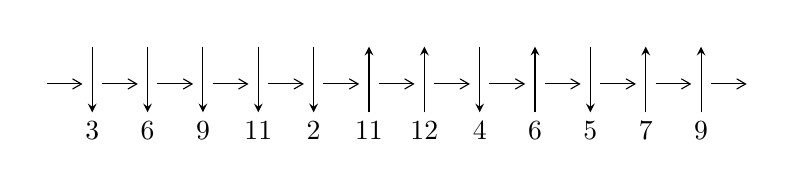
\begin{tikzpicture}[x=20pt, y=17pt]
	% nodes
	\node (C0) at (0, 0) {};
	\node (C1) at (1, 0) {};
	\node (C1U) at (1, +1) {};
	\node (C1D) at (1, -1) {3};

	\node (C2) at (2, 0) {};
	\node (C2U) at (2, +1) {};
	\node (C2D) at (2, -1) {6};

	\node (C3) at (3, 0) {};
	\node (C3U) at (3, +1) {};
	\node (C3D) at (3, -1) {9};

	\node (C4) at (4, 0) {};
	\node (C4U) at (4, +1) {};
	\node (C4D) at (4, -1) {11};

	\node (C5) at (5, 0) {};
	\node (C5U) at (5, +1) {};
	\node (C5D) at (5, -1) {2};

	\node (C6) at (6, 0) {};
	\node (C6U) at (6, +1) {};
	\node (C6D) at (6, -1) {11};

	\node (C7) at (7, 0) {};
	\node (C7U) at (7, +1) {};
	\node (C7D) at (7, -1) {12};

	\node (C8) at (8, 0) {};
	\node (C8U) at (8, +1) {};
	\node (C8D) at (8, -1) {4};

	\node (C9) at (9, 0) {};
	\node (C9U) at (9, +1) {};
	\node (C9D) at (9, -1) {6};

	\node (C10) at (10, 0) {};
	\node (C10U) at (10, +1) {};
	\node (C10D) at (10, -1) {5};

	\node (C11) at (11, 0) {};
	\node (C11U) at (11, +1) {};
	\node (C11D) at (11, -1) {7};

	\node (C12) at (12, 0) {};
	\node (C12U) at (12, +1) {};
	\node (C12D) at (12, -1) {9};
	\node (C13) at (13, 0) {};

	% arrows
	\draw[->,>={angle 60}]
	(C0) edge (C1) (C1) edge (C2) (C2) edge (C3) (C3) edge (C4) (C4) edge (C5) (C5) edge (C6) (C6) edge (C7) (C7) edge (C8) (C8) edge (C9) (C9) edge (C10) (C10) edge (C11) (C11) edge (C12) (C12) edge (C13) ;	\draw[->,>=stealth]
	(C1U) edge (C1D) (C2U) edge (C2D) (C3U) edge (C3D) (C4U) edge (C4D) (C5U) edge (C5D) (C6D) edge (C6U) (C7D) edge (C7U) (C8U) edge (C8D) (C9D) edge (C9U) (C10U) edge (C10D) (C11D) edge (C11U) (C12D) edge (C12U) ;
	\end{tikzpicture} \\
\hhline{~~} \\& 
\textbf{Solving Sequence} \\ \cline{2-2} 
 &
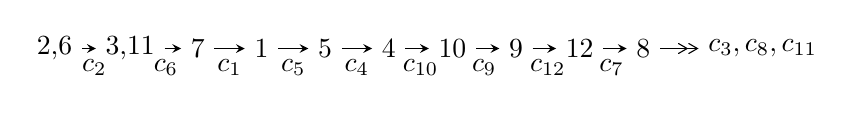
\begin{tikzpicture}[x=23pt, y=7pt]
	% node
	\node (A0) at (-1/8, 0) {2,6};
	\node (A1) at (17/16, 0) {3,11};
	\node (A2) at (17/8, 0) {7};
	\node (A3) at (25/8, 0) {1};
	\node (A4) at (33/8, 0) {5};
	\node (A5) at (41/8, 0) {4};
	\node (A6) at (49/8, 0) {10};
	\node (A7) at (57/8, 0) {9};
	\node (A8) at (65/8, 0) {12};
	\node (A9) at (73/8, 0) {8};
	\node (C1) at (1/2, -1) {$c_{2}$};
	\node (C2) at (13/8, -1) {$c_{6}$};
	\node (C3) at (21/8, -1) {$c_{1}$};
	\node (C4) at (29/8, -1) {$c_{5}$};
	\node (C5) at (37/8, -1) {$c_{4}$};
	\node (C6) at (45/8, -1) {$c_{10}$};
	\node (C7) at (53/8, -1) {$c_{9}$};
	\node (C8) at (61/8, -1) {$c_{12}$};
	\node (C9) at (69/8, -1) {$c_{7}$};
	\node (A10) at (11, 0) {$c_{3},c_{8},c_{11}$};

	% edge
	\draw[->,>=stealth]	
	(A0) edge (A1) (A1) edge (A2) (A2) edge (A3) (A3) edge (A4) (A4) edge (A5) (A5) edge (A6) (A6) edge (A7) (A7) edge (A8) (A8) edge (A9) ;
	\draw[->>,>={angle 60}]	
	(A9) edge (A10);
\end{tikzpicture} \\ 

\end{tabular} \\

\footnotetext{
The image of knot diagram is generated by the software ``\textbf{Draw programme}" developed by Andrew Bartholomew(\url{http://www.layer8.co.uk/maths/draw/index.htm\#Running-draw}), where we modified some parts for our purpose(\url{https://github.com/CATsTAILs/LinksPainter}).
}\phantom \\ \newline 
\centering \textbf{Ideals for irreducible components\footnotemark of $X_{\text{par}}$} 
 
\begin{align*}
I^u_{1}&=\langle 
u^8-2 u^7+3 u^6-3 u^5+4 u^4-3 u^3+2 u^2+b- u,\;u^6-2 u^5+2 u^4- u^3+2 u^2+a-2 u,\\
\phantom{I^u_{1}}&\phantom{= \langle  }u^9-3 u^8+5 u^7-5 u^6+6 u^5-7 u^4+6 u^3-2 u^2+u-1\rangle \\
I^u_{2}&=\langle 
u^6+2 u^5+u^4-2 u^3-2 u^2+b,\;u^6+2 u^5+2 u^4- u^3-2 u^2+a-2 u,\;u^7+2 u^6+2 u^5- u^4- u^3- u^2-1\rangle \\
\\
\end{align*}
\raggedright * 2 irreducible components of $\dim_{\mathbb{C}}=0$, with total 16 representations.\\
\footnotetext{All coefficients of polynomials are rational numbers. But the coefficients are sometimes approximated in decimal forms when there is not enough margin.}
\newpage
\renewcommand{\arraystretch}{1}
\centering \section*{I. $I^u_{1}= \langle u^8-2 u^7+\cdots+b- u,\;u^6-2 u^5+2 u^4- u^3+2 u^2+a-2 u,\;u^9-3 u^8+\cdots+u-1 \rangle$}
\flushleft \textbf{(i) Arc colorings}\\
\begin{tabular}{m{7pt} m{180pt} m{7pt} m{180pt} }
\flushright $a_{2}=$&$\begin{pmatrix}1\\0\end{pmatrix}$ \\
\flushright $a_{6}=$&$\begin{pmatrix}0\\u\end{pmatrix}$ \\
\flushright $a_{3}=$&$\begin{pmatrix}1\\u^2\end{pmatrix}$ \\
\flushright $a_{11}=$&$\begin{pmatrix}- u^6+2 u^5-2 u^4+u^3-2 u^2+2 u\\- u^8+2 u^7-3 u^6+3 u^5-4 u^4+3 u^3-2 u^2+u\end{pmatrix}$ \\
\flushright $a_{7}=$&$\begin{pmatrix}- u^7+u^6- u^5+u^4-3 u^3+2 u^2- u+1\\- u^8+u^7- u^6+u^5-2 u^4+u^2+u\end{pmatrix}$ \\
\flushright $a_{1}=$&$\begin{pmatrix}- u^2+1\\- u^4\end{pmatrix}$ \\
\flushright $a_{5}=$&$\begin{pmatrix}u\\u\end{pmatrix}$ \\
\flushright $a_{4}=$&$\begin{pmatrix}u^8-2 u^7+2 u^6-2 u^5+3 u^4-3 u^3+u^2+1\\u^8-3 u^7+3 u^6-3 u^5+4 u^4-5 u^3+2 u^2+1\end{pmatrix}$ \\
\flushright $a_{10}=$&$\begin{pmatrix}u^7-2 u^6+3 u^5-3 u^4+4 u^3-3 u^2+2 u-1\\- u^8+3 u^7-4 u^6+4 u^5-5 u^4+6 u^3-3 u^2+u-1\end{pmatrix}$ \\
\flushright $a_{9}=$&$\begin{pmatrix}u^7-2 u^6+3 u^5-3 u^4+4 u^3-3 u^2+2 u-1\\u^7-2 u^6+2 u^5- u^4+2 u^3-2 u^2\end{pmatrix}$ \\
\flushright $a_{12}=$&$\begin{pmatrix}u^7- u^6+u^5- u^4+2 u^3-2 u^2+u\\u^8- u^7+u^6- u^5+u^4- u^2\end{pmatrix}$ \\
\flushright $a_{8}=$&$\begin{pmatrix}-2 u^7+4 u^6-5 u^5+4 u^4-8 u^3+5 u^2-2 u+2\\- u^8+u^7- u^5-3 u^4+2 u^2+u\end{pmatrix}$\\&\end{tabular}
\flushleft \textbf{(ii) Obstruction class $= -1$}\\~\\
\flushleft \textbf{(iii) Cusp Shapes $= -5 u^8+12 u^7-17 u^6+12 u^5-20 u^4+20 u^3-13 u^2-6 u-3$}\\~\\
\newpage\renewcommand{\arraystretch}{1}
\flushleft \textbf{(iv) u-Polynomials at the component}\newline \\
\begin{tabular}{m{50pt}|m{274pt}}
Crossings & \hspace{64pt}u-Polynomials at each crossing \\
\hline $$\begin{aligned}c_{1}\end{aligned}$$&$\begin{aligned}
&u^9- u^8+7 u^7-5 u^6+16 u^5-7 u^4+10 u^3+6 u^2-3 u+1
\end{aligned}$\\
\hline $$\begin{aligned}c_{2},c_{5}\end{aligned}$$&$\begin{aligned}
&u^9+3 u^8+5 u^7+5 u^6+6 u^5+7 u^4+6 u^3+2 u^2+u+1
\end{aligned}$\\
\hline $$\begin{aligned}c_{3},c_{4},c_{8}\\c_{10}\end{aligned}$$&$\begin{aligned}
&u^9-2 u^7+4 u^6+17 u^5+9 u^4+9 u^3+2 u^2+2 u+1
\end{aligned}$\\
\hline $$\begin{aligned}c_{6},c_{7},c_{11}\end{aligned}$$&$\begin{aligned}
&u^9+8 u^8+27 u^7+46 u^6+33 u^5-10 u^4-27 u^3- u^2+14 u+4
\end{aligned}$\\
\hline $$\begin{aligned}c_{9},c_{12}\end{aligned}$$&$\begin{aligned}
&u^9-4 u^8+8 u^7-3 u^6-2 u^4+24 u^3-23 u^2+9 u+1
\end{aligned}$\\
\hline
\end{tabular}\\~\\
\newpage\renewcommand{\arraystretch}{1}
\flushleft \textbf{(v) Riley Polynomials at the component}\newline \\
\begin{tabular}{m{50pt}|m{274pt}}
Crossings & \hspace{64pt}Riley Polynomials at each crossing \\
\hline $$\begin{aligned}c_{1}\end{aligned}$$&$\begin{aligned}
&y^9+13 y^8+71 y^7+205 y^6+332 y^5+291 y^4+98 y^3-82 y^2-3 y-1
\end{aligned}$\\
\hline $$\begin{aligned}c_{2},c_{5}\end{aligned}$$&$\begin{aligned}
&y^9+y^8+7 y^7+5 y^6+16 y^5+7 y^4+10 y^3-6 y^2-3 y-1
\end{aligned}$\\
\hline $$\begin{aligned}c_{3},c_{4},c_{8}\\c_{10}\end{aligned}$$&$\begin{aligned}
&y^9-4 y^8+38 y^7-66 y^6+185 y^5+201 y^4+105 y^3+14 y^2-1
\end{aligned}$\\
\hline $$\begin{aligned}c_{6},c_{7},c_{11}\end{aligned}$$&$\begin{aligned}
&y^9-10 y^8+\cdots+204 y-16
\end{aligned}$\\
\hline $$\begin{aligned}c_{9},c_{12}\end{aligned}$$&$\begin{aligned}
&y^9+40 y^7+23 y^6+206 y^5+10 y^4+490 y^3-93 y^2+127 y-1
\end{aligned}$\\
\hline
\end{tabular}\\~\\
\newpage\flushleft \textbf{(vi) Complex Volumes and Cusp Shapes}
$$\begin{array}{c|c|c}  
\text{Solutions to }I^u_{1}& \I (\text{vol} + \sqrt{-1}CS) & \text{Cusp shape}\\
 \hline 
\begin{aligned}
u &= -0.543663 + 0.958634 I \\
a &= -0.62928 - 1.29649 I \\
b &= -1.044710 - 0.790946 I\end{aligned}
 & \phantom{-}8.80377 + 2.34106 I & \phantom{-}3.55048 - 3.71378 I \\ \hline\begin{aligned}
u &= -0.543663 - 0.958634 I \\
a &= -0.62928 + 1.29649 I \\
b &= -1.044710 + 0.790946 I\end{aligned}
 & \phantom{-}8.80377 - 2.34106 I & \phantom{-}3.55048 + 3.71378 I \\ \hline\begin{aligned}
u &= \phantom{-}0.780042\phantom{ +0.000000I} \\
a &= \phantom{-}0.429639\phantom{ +0.000000I} \\
b &= -0.0889832\phantom{ +0.000000I}\end{aligned}
 & -1.02700\phantom{ +0.000000I} & -12.4430\phantom{ +0.000000I} \\ \hline\begin{aligned}
u &= \phantom{-}1.022250 + 0.813773 I \\
a &= \phantom{-}1.249250 - 0.023619 I \\
b &= \phantom{-}0.74446 + 1.23201 I\end{aligned}
 & -2.68542 + 1.09922 I & \phantom{-}0.831621 - 0.481760 I \\ \hline\begin{aligned}
u &= \phantom{-}1.022250 - 0.813773 I \\
a &= \phantom{-}1.249250 + 0.023619 I \\
b &= \phantom{-}0.74446 - 1.23201 I\end{aligned}
 & -2.68542 - 1.09922 I & \phantom{-}0.831621 + 0.481760 I \\ \hline\begin{aligned}
u &= \phantom{-}0.877200 + 1.062120 I \\
a &= \phantom{-}0.148693 - 1.372070 I \\
b &= \phantom{-}1.77486 - 1.66508 I\end{aligned}
 & -1.87595 - 8.01095 I & \phantom{-}1.68345 + 4.08979 I \\ \hline\begin{aligned}
u &= \phantom{-}0.877200 - 1.062120 I \\
a &= \phantom{-}0.148693 + 1.372070 I \\
b &= \phantom{-}1.77486 + 1.66508 I\end{aligned}
 & -1.87595 + 8.01095 I & \phantom{-}1.68345 - 4.08979 I \\ \hline\begin{aligned}
u &= -0.245807 + 0.515171 I \\
a &= \phantom{-}0.016526 + 1.227710 I \\
b &= \phantom{-}0.569881 + 0.456696 I\end{aligned}
 & \phantom{-}1.20590 + 0.78253 I & \phantom{-}4.15601 - 2.65874 I \\ \hline\begin{aligned}
u &= -0.245807 - 0.515171 I \\
a &= \phantom{-}0.016526 - 1.227710 I \\
b &= \phantom{-}0.569881 - 0.456696 I\end{aligned}
 & \phantom{-}1.20590 - 0.78253 I & \phantom{-}4.15601 + 2.65874 I\\
 \hline 
 \end{array}$$\newpage\newpage\renewcommand{\arraystretch}{1}
\centering \section*{II. $I^u_{2}= \langle u^6+2 u^5+u^4-2 u^3-2 u^2+b,\;u^6+2 u^5+2 u^4- u^3-2 u^2+a-2 u,\;u^7+2 u^6+2 u^5- u^4- u^3- u^2-1 \rangle$}
\flushleft \textbf{(i) Arc colorings}\\
\begin{tabular}{m{7pt} m{180pt} m{7pt} m{180pt} }
\flushright $a_{2}=$&$\begin{pmatrix}1\\0\end{pmatrix}$ \\
\flushright $a_{6}=$&$\begin{pmatrix}0\\u\end{pmatrix}$ \\
\flushright $a_{3}=$&$\begin{pmatrix}1\\u^2\end{pmatrix}$ \\
\flushright $a_{11}=$&$\begin{pmatrix}- u^6-2 u^5-2 u^4+u^3+2 u^2+2 u\\- u^6-2 u^5- u^4+2 u^3+2 u^2\end{pmatrix}$ \\
\flushright $a_{7}=$&$\begin{pmatrix}u^6+3 u^5+4 u^4-3 u^2-3 u\\u^6+2 u^5+2 u^4-2 u^3-2 u^2+1\end{pmatrix}$ \\
\flushright $a_{1}=$&$\begin{pmatrix}- u^2+1\\- u^4\end{pmatrix}$ \\
\flushright $a_{5}=$&$\begin{pmatrix}u\\u\end{pmatrix}$ \\
\flushright $a_{4}=$&$\begin{pmatrix}u^5+2 u^4+2 u^3- u^2- u-1\\u^6+2 u^5+2 u^4- u^3- u^2- u\end{pmatrix}$ \\
\flushright $a_{10}=$&$\begin{pmatrix}- u^5-2 u^4- u^3+2 u^2+2 u\\- u^5- u^4+2 u^2\end{pmatrix}$ \\
\flushright $a_{9}=$&$\begin{pmatrix}- u^5-2 u^4- u^3+2 u^2+2 u\\u^3+u^2-1\end{pmatrix}$ \\
\flushright $a_{12}=$&$\begin{pmatrix}u^6+3 u^5+4 u^4+u^3-3 u^2-3 u-1\\u^6+2 u^5+u^4-2 u^3-2 u^2- u+1\end{pmatrix}$ \\
\flushright $a_{8}=$&$\begin{pmatrix}- u^5-2 u^4-2 u^3+u^2+2 u+2\\- u^4+u^2+2 u-1\end{pmatrix}$\\&\end{tabular}
\flushleft \textbf{(ii) Obstruction class $= 1$}\\~\\
\flushleft \textbf{(iii) Cusp Shapes $= 3 u^6+5 u^5+3 u^4-5 u^3- u^2- u+3$}\\~\\
\newpage\renewcommand{\arraystretch}{1}
\flushleft \textbf{(iv) u-Polynomials at the component}\newline \\
\begin{tabular}{m{50pt}|m{274pt}}
Crossings & \hspace{64pt}u-Polynomials at each crossing \\
\hline $$\begin{aligned}c_{1}\end{aligned}$$&$\begin{aligned}
&u^7+6 u^5- u^4+3 u^3-3 u^2-2 u-1
\end{aligned}$\\
\hline $$\begin{aligned}c_{2}\end{aligned}$$&$\begin{aligned}
&u^7+2 u^6+2 u^5- u^4- u^3- u^2-1
\end{aligned}$\\
\hline $$\begin{aligned}c_{3},c_{10}\end{aligned}$$&$\begin{aligned}
&u^7+u^6+4 u^5+3 u^4+6 u^3+2 u^2+3 u-1
\end{aligned}$\\
\hline $$\begin{aligned}c_{4},c_{8}\end{aligned}$$&$\begin{aligned}
&u^7- u^6+4 u^5-3 u^4+6 u^3-2 u^2+3 u+1
\end{aligned}$\\
\hline $$\begin{aligned}c_{5}\end{aligned}$$&$\begin{aligned}
&u^7-2 u^6+2 u^5+u^4- u^3+u^2+1
\end{aligned}$\\
\hline $$\begin{aligned}c_{6},c_{7}\end{aligned}$$&$\begin{aligned}
&u^7-5 u^5+7 u^3- u+1
\end{aligned}$\\
\hline $$\begin{aligned}c_{9},c_{12}\end{aligned}$$&$\begin{aligned}
&u^7+3 u^6-8 u^4-4 u^3+8 u^2+4 u-3
\end{aligned}$\\
\hline $$\begin{aligned}c_{11}\end{aligned}$$&$\begin{aligned}
&u^7-5 u^5+7 u^3- u-1
\end{aligned}$\\
\hline
\end{tabular}\\~\\
\newpage\renewcommand{\arraystretch}{1}
\flushleft \textbf{(v) Riley Polynomials at the component}\newline \\
\begin{tabular}{m{50pt}|m{274pt}}
Crossings & \hspace{64pt}Riley Polynomials at each crossing \\
\hline $$\begin{aligned}c_{1}\end{aligned}$$&$\begin{aligned}
&y^7+12 y^6+42 y^5+31 y^4-21 y^3-23 y^2-2 y-1
\end{aligned}$\\
\hline $$\begin{aligned}c_{2},c_{5}\end{aligned}$$&$\begin{aligned}
&y^7+6 y^5- y^4+3 y^3-3 y^2-2 y-1
\end{aligned}$\\
\hline $$\begin{aligned}c_{3},c_{4},c_{8}\\c_{10}\end{aligned}$$&$\begin{aligned}
&y^7+7 y^6+22 y^5+41 y^4+50 y^3+38 y^2+13 y-1
\end{aligned}$\\
\hline $$\begin{aligned}c_{6},c_{7},c_{11}\end{aligned}$$&$\begin{aligned}
&y^7-10 y^6+39 y^5-72 y^4+59 y^3-14 y^2+y-1
\end{aligned}$\\
\hline $$\begin{aligned}c_{9},c_{12}\end{aligned}$$&$\begin{aligned}
&y^7-9 y^6+40 y^5-104 y^4+162 y^3-144 y^2+64 y-9
\end{aligned}$\\
\hline
\end{tabular}\\~\\
\newpage\flushleft \textbf{(vi) Complex Volumes and Cusp Shapes}
$$\begin{array}{c|c|c}  
\text{Solutions to }I^u_{2}& \I (\text{vol} + \sqrt{-1}CS) & \text{Cusp shape}\\
 \hline 
\begin{aligned}
u &= -0.679131 + 0.739231 I \\
a &= -0.090421 + 0.468757 I \\
b &= \phantom{-}1.067080 - 0.219644 I\end{aligned}
 & \phantom{-}4.71019 + 2.40933 I & \phantom{-}0.29860 - 3.62563 I \\ \hline\begin{aligned}
u &= -0.679131 - 0.739231 I \\
a &= -0.090421 - 0.468757 I \\
b &= \phantom{-}1.067080 + 0.219644 I\end{aligned}
 & \phantom{-}4.71019 - 2.40933 I & \phantom{-}0.29860 + 3.62563 I \\ \hline\begin{aligned}
u &= \phantom{-}0.939920\phantom{ +0.000000I} \\
a &= \phantom{-}0.759448\phantom{ +0.000000I} \\
b &= \phantom{-}0.490461\phantom{ +0.000000I}\end{aligned}
 & -0.502424\phantom{ +0.000000I} & \phantom{-}5.10270\phantom{ +0.000000I} \\ \hline\begin{aligned}
u &= \phantom{-}0.273857 + 0.616814 I \\
a &= -0.63288 + 2.30893 I \\
b &= -1.49346 + 0.77301 I\end{aligned}
 & \phantom{-}9.14166 - 1.05666 I & \phantom{-}5.26558 - 1.27318 I \\ \hline\begin{aligned}
u &= \phantom{-}0.273857 - 0.616814 I \\
a &= -0.63288 - 2.30893 I \\
b &= -1.49346 - 0.77301 I\end{aligned}
 & \phantom{-}9.14166 + 1.05666 I & \phantom{-}5.26558 + 1.27318 I \\ \hline\begin{aligned}
u &= -1.06469 + 1.08838 I \\
a &= -0.656418 - 0.759679 I \\
b &= -1.318850 - 0.288008 I\end{aligned}
 & \phantom{-}11.07340 + 3.97449 I & \phantom{-}4.88445 - 3.30547 I \\ \hline\begin{aligned}
u &= -1.06469 - 1.08838 I \\
a &= -0.656418 + 0.759679 I \\
b &= -1.318850 + 0.288008 I\end{aligned}
 & \phantom{-}11.07340 - 3.97449 I & \phantom{-}4.88445 + 3.30547 I\\
 \hline 
 \end{array}$$\newpage
\newpage\renewcommand{\arraystretch}{1}
\centering \section*{ III. u-Polynomials}
\begin{tabular}{m{50pt}|m{274pt}}
Crossings & \hspace{64pt}u-Polynomials at each crossing \\
\hline $$\begin{aligned}c_{1}\end{aligned}$$&$\begin{aligned}
&(u^7+6 u^5- u^4+3 u^3-3 u^2-2 u-1)\\
&\cdot(u^9- u^8+7 u^7-5 u^6+16 u^5-7 u^4+10 u^3+6 u^2-3 u+1)
\end{aligned}$\\
\hline $$\begin{aligned}c_{2}\end{aligned}$$&$\begin{aligned}
&(u^7+2 u^6+2 u^5- u^4- u^3- u^2-1)\\
&\cdot(u^9+3 u^8+5 u^7+5 u^6+6 u^5+7 u^4+6 u^3+2 u^2+u+1)
\end{aligned}$\\
\hline $$\begin{aligned}c_{3},c_{10}\end{aligned}$$&$\begin{aligned}
&(u^7+u^6+4 u^5+3 u^4+6 u^3+2 u^2+3 u-1)\\
&\cdot(u^9-2 u^7+4 u^6+17 u^5+9 u^4+9 u^3+2 u^2+2 u+1)
\end{aligned}$\\
\hline $$\begin{aligned}c_{4},c_{8}\end{aligned}$$&$\begin{aligned}
&(u^7- u^6+4 u^5-3 u^4+6 u^3-2 u^2+3 u+1)\\
&\cdot(u^9-2 u^7+4 u^6+17 u^5+9 u^4+9 u^3+2 u^2+2 u+1)
\end{aligned}$\\
\hline $$\begin{aligned}c_{5}\end{aligned}$$&$\begin{aligned}
&(u^7-2 u^6+2 u^5+u^4- u^3+u^2+1)\\
&\cdot(u^9+3 u^8+5 u^7+5 u^6+6 u^5+7 u^4+6 u^3+2 u^2+u+1)
\end{aligned}$\\
\hline $$\begin{aligned}c_{6},c_{7}\end{aligned}$$&$\begin{aligned}
&(u^7-5 u^5+7 u^3- u+1)\\
&\cdot(u^9+8 u^8+27 u^7+46 u^6+33 u^5-10 u^4-27 u^3- u^2+14 u+4)
\end{aligned}$\\
\hline $$\begin{aligned}c_{9},c_{12}\end{aligned}$$&$\begin{aligned}
&(u^7+3 u^6-8 u^4-4 u^3+8 u^2+4 u-3)\\
&\cdot(u^9-4 u^8+8 u^7-3 u^6-2 u^4+24 u^3-23 u^2+9 u+1)
\end{aligned}$\\
\hline $$\begin{aligned}c_{11}\end{aligned}$$&$\begin{aligned}
&(u^7-5 u^5+7 u^3- u-1)\\
&\cdot(u^9+8 u^8+27 u^7+46 u^6+33 u^5-10 u^4-27 u^3- u^2+14 u+4)
\end{aligned}$\\
\hline
\end{tabular}\newpage\renewcommand{\arraystretch}{1}
\centering \section*{ IV. Riley Polynomials}
\begin{tabular}{m{50pt}|m{274pt}}
Crossings & \hspace{64pt}Riley Polynomials at each crossing \\
\hline $$\begin{aligned}c_{1}\end{aligned}$$&$\begin{aligned}
&(y^7+12 y^6+42 y^5+31 y^4-21 y^3-23 y^2-2 y-1)\\
&\cdot(y^9+13 y^8+71 y^7+205 y^6+332 y^5+291 y^4+98 y^3-82 y^2-3 y-1)
\end{aligned}$\\
\hline $$\begin{aligned}c_{2},c_{5}\end{aligned}$$&$\begin{aligned}
&(y^7+6 y^5- y^4+3 y^3-3 y^2-2 y-1)\\
&\cdot(y^9+y^8+7 y^7+5 y^6+16 y^5+7 y^4+10 y^3-6 y^2-3 y-1)
\end{aligned}$\\
\hline $$\begin{aligned}c_{3},c_{4},c_{8}\\c_{10}\end{aligned}$$&$\begin{aligned}
&(y^7+7 y^6+22 y^5+41 y^4+50 y^3+38 y^2+13 y-1)\\
&\cdot(y^9-4 y^8+38 y^7-66 y^6+185 y^5+201 y^4+105 y^3+14 y^2-1)
\end{aligned}$\\
\hline $$\begin{aligned}c_{6},c_{7},c_{11}\end{aligned}$$&$\begin{aligned}
&(y^7-10 y^6+39 y^5-72 y^4+59 y^3-14 y^2+y-1)\\
&\cdot(y^9-10 y^8+\cdots+204 y-16)
\end{aligned}$\\
\hline $$\begin{aligned}c_{9},c_{12}\end{aligned}$$&$\begin{aligned}
&(y^7-9 y^6+40 y^5-104 y^4+162 y^3-144 y^2+64 y-9)\\
&\cdot(y^9+40 y^7+23 y^6+206 y^5+10 y^4+490 y^3-93 y^2+127 y-1)
\end{aligned}$\\
\hline
\end{tabular}
\vskip 2pc
\end{document}